\chapter{Introduction}
\label{chapter:introduction}

Reinforcement learning has been shown to solve complex problems. Recently it has been used with great success by google DeepMind playing Atari games. The success is great but understanding the basic of some of these frameworks/algorithms can be daunting. In this post I hope to eliminate some of the mental entropy cause by trying to understand how and why the algorithms work. I will focus on Logistic Regression as it is a simple and if we can understand this model then more complex models are far easier to comprehend. 
Going into this I do expect that the reader has some math background. They should understand what a gradient is, and a little about RL in particular what a policy is and how Q-Learning works. I learnt this topic by taking apart algorithms designed for classification, some of this might seep into the discussion.

\section{Framework}

These examples are coded in Python. I am not saying it is the best language in the world but I think in this case it helps the reader (including myself) understand what is going on in the program better.

\subsection{Theano}

There is also heavy use of a Python library called Theano~\cite{Bastien-Theano-2012}. This library is fantastic, in my opinion. The library seems to be a symbolic math computing library with support for using the GPU (GPU not used in this work). Using Theano is more like creating a data flow model where variables are vectors/matricies.

\paragraph{Example:} Create a simple function $f(x)=x+x^{10}$

\begin{lstlisting}
import theano
a = theano.tensor.vector() # declare variable
out = a + a ** 10 # build symbolic expression
f = theano.function([a], out)   # compile function
print(f([0, 1, 2]))
out >> [    0.     2.  1026.]
\end{lstlisting}
 

  
This example shows some of those features. First you need to declare the type of variable that will be used, something like vector or matrix. Create a symbolic mathematical expression that you want to compute over the variable type. Next you compile the function, this part almost literally compiles a C function in the background that data will be fed through to get output.

\subsection{The Environment}
I wanted to use a very simple environment to demonstrate the workings of RL. I decided on a 2D navigation game because you can visualize the policy so nicely.
Navigation Game
The game consists of an agent, a goal and a square 2D world the agent navigates in. The state of the game is shown on the left and the current policy for the agent is shown on the right.

\begin{figure}
	\centering
	\label{figure:navigation-game}
	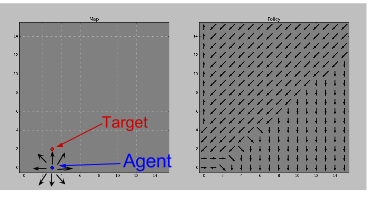
\includegraphics[width=0.9\linewidth]{../images/NavigationGame.png}
	\caption{This figure illustrates the navigation game that will be used in the examples. The state of the game is 
	on the left, where the actions the agent has available is also shown. The current policy for the agent is shown
	on the right. The arrows correspond to the action the agent would take at that location.}
\end{figure}

The agent can move in any of $8$ directions, as is shown on the left. The target location of the agent is the red dot. 
Reinforcement Learning
One key difference when using Logistic Regression for RL instead of classification is the data. In classification the data is pre-labled with the correct class that we want the model to predict. In RL there is no pre-labeled data. We have to generate data ourselves and this data has a reward signal that should be maximized not a class.
Bellman Error
It is not just the reward signal we want to maximize but the discounted future reward 
\begin{equation}
	\qValueFunction{\state_{0}}{\action_{0}}{} = \discountFactor^{0} r_{0} + \discountFactor^{1} r_{1} + \cdots + \discountFactor^{t-1} r_{t-1} + \discountFactor^{t} r_{t}.
\end{equation}

 This is done minimizing the Bellman Error 
 \begin{equation}
 	\bellmanError = (\reward + \discountFactor \argmax_{a'} \qValueFunction{\state}{a'}{})−\qValueFunction{\state}{\action}{}.
 \end{equation}
